\section{Motor controller}
In the following paragraphs the hardware implemented for the motor controller for AU2 will be discussed. 

Even though the PCB is dubbed motor controller it consists of a large variety of subsystems. The list is comprised of: 

\begin{itemize}
	\item{Horn}
	\item{Distribution Block}
	\item{Motor Controller Unit}
	\item{Speedometer}
	\item{Interface}
	\item{Motor Controller}
	\item{Measurements}
	\item{SDcard}
	\item{CAN-transceiver}
\end{itemize}

Where each item on the above list requires more or less circuit for operation. 

When designing the hardware for the motor controller to consist of, the most time-consuming were the distribution block, the actual motor controller and the CAN-transceiver. The reason for time spend on these matters is purely on a current consumption matter by trying to find that special component, that will be more efficient than the other. 

The solution found for the distribution block is the IC LT8300\cite{LT8300} from linear technologies. This IC is chosen for two reasons; The first being, that the previous car that took part in Shell Eco Marathon used this, but the more convincing argument for using this specific IC is the high efficiency as seen on figure \vref{fig:LT8300}. The efficiency varies with load current and peaks at around 85\% at 150mA load.  

\begin{figure}[H]
	\centering
	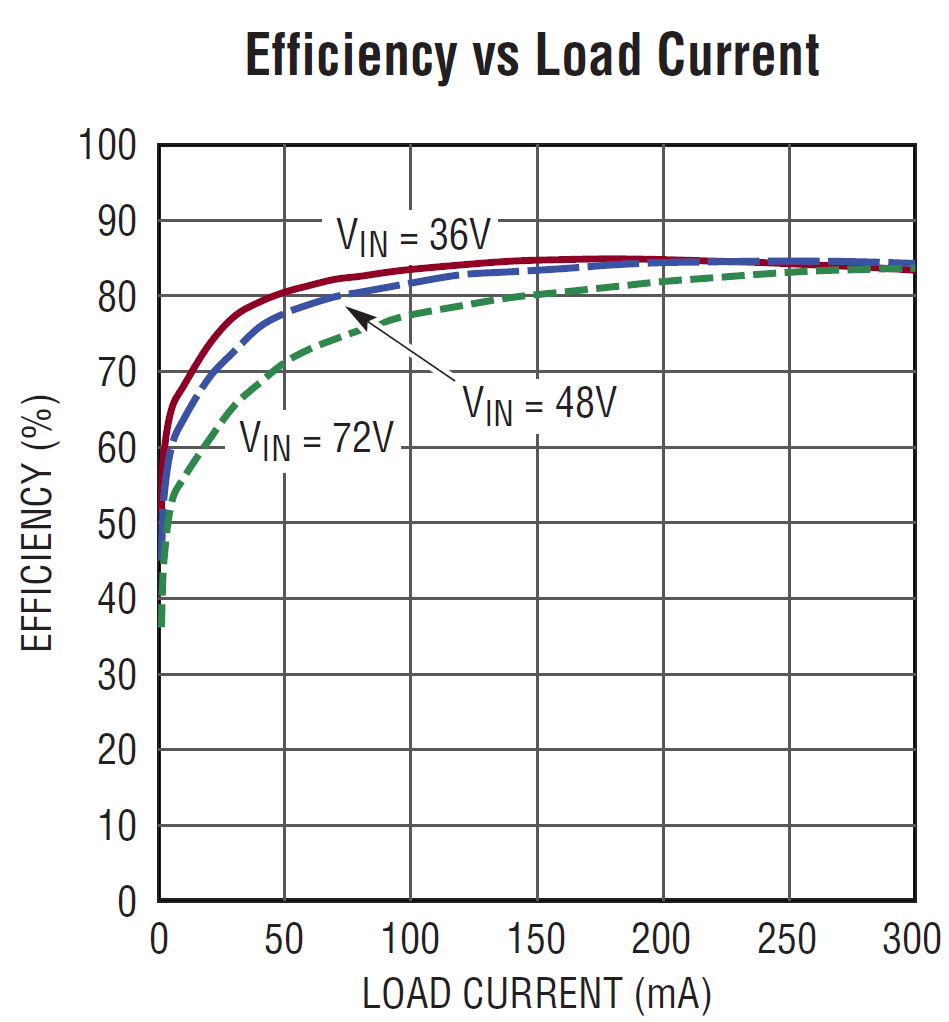
\includegraphics[width=0.5\linewidth]{Hardware/Pictures/LT8300}
	\caption{Efficiency diagram for the LT8300}
	\label{fig:LT8300}
\end{figure}

The solution found for the CAN-transceiver was an IC from Texas instruments, SN65HVD1040\cite{CAN}. This CAN transceiver is a very low power transceiver with the option to use bus wakeup(not implemented). This transceiver was chosen solely for its low current consumption as seen on figure \vref{fig:CAN}. 

\begin{figure}[H]
	\centering
	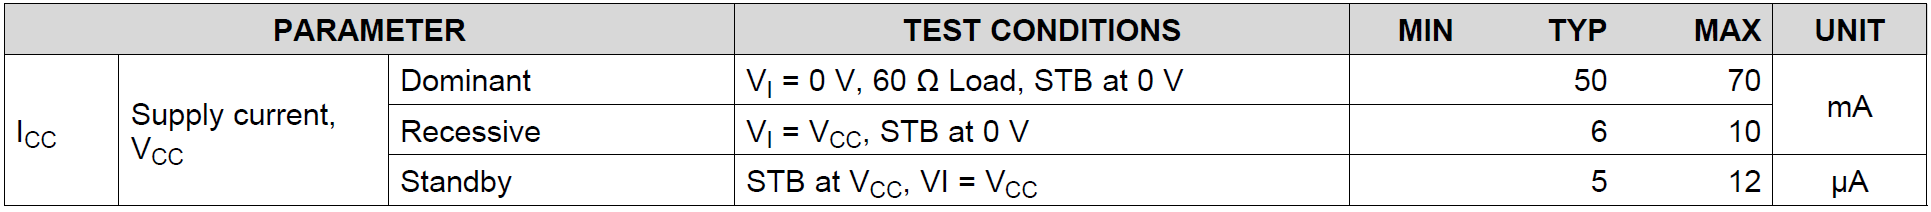
\includegraphics[width=1\linewidth]{Hardware/Pictures/CAN}
	\caption{SN65HVD1040 supply current}
	\label{fig:CAN}
\end{figure}

The motorcontroller consist of a series of component with the important one being the MOSFeT at use. The MOSFET chosen to control the motor is the IRFB7530\cite{IRFB7530} from International rectifiers. As seen on figure \vref{fig:MOSFET} the on resistance for the MOSFET is a mere \SI{2}{\milli \ohm} at max. This means there is a small current dissipation when the MOSFET is conducting. This also means that the gate capacitance is high, but this is compensated for by the MOSFET driver.  

\begin{figure}[H]
	\centering
	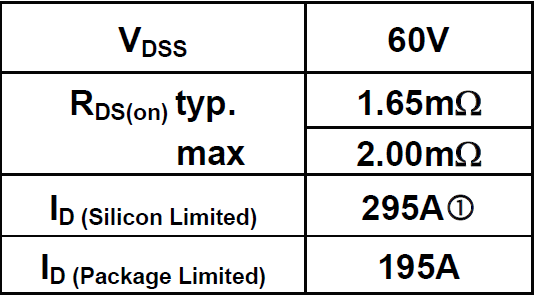
\includegraphics[width=0.5\linewidth]{Hardware/Pictures/IRFB7530}
	\caption{IRFB7530 Specifications}
	\label{fig:MOSFET}
\end{figure}

Furthermore all the aforementioned components is qualified for use in automotive use, which means that they have been exposed to a series of test, to ensure that they are reliant and sturdy enough to withstand the possibility of extra outer forces when placed in an automotive vehicle. 

The hardware developed for the motor controller is realised on a PCB. Doing so requires extra some extra time to realise the designed circuit, as using the ultiboard software requires some adaption. But when then print layout is completed, the implementation is eased as soldering the PCB becomes easier. The downside to using a PCB instead of a breadboard is the added complexity when switching components. That sets some demands for the design to be thouroughly tested before implementing it on a PCB.

Even though implementing the designed circuit on a PCB has it downsides, the plus sides weighs it up. This is because SMD components make the implementation phase better in the sense that they physically are a lot smaller and by that decreases the size of the PCB. Furthermore implementing the circuit onto a PCB gives a series of design features such as minimizing trace to decoupling capacitors. Furthermore it gives the designer a selection amongst many connectors to be used on the PCB. 

